\documentclass[
a4paper,
11pt,
english
]{report}

\usepackage[utf8]{inputenc} % Required for inputting international characters
\usepackage[T1]{fontenc} % Output font encoding for international characters

\usepackage{mathpazo} % Use the Palatino font by default

\usepackage[backend=bibtex,style=authoryear,natbib=true]{biblatex} % Use the bibtex backend with the authoryear citation style (which resembles APA)

\addbibresource{example.bib} % The filename of the bibliography

\usepackage[autostyle=true]{csquotes} % Required to generate language-dependent quotes in the bibliography

\usepackage[left=1in, right=1in]{geometry}
\linespread{1.5}
\usepackage[utf8]{inputenc}
\usepackage{graphicx}
\usepackage{listings}
\usepackage{longtable}
\usepackage{xcolor}
\usepackage{color}
\usepackage{hyperref}

\newenvironment{myitemize}{
    \begin{itemize}
    \setlength{\itemsep}{0pt}
    \setlength{\parskip}{0pt}
    \setlength{\parsep}{0pt}
}{\end{itemize}}

%----------------------------------------------------------------------------------------
%	MARGIN SETTINGS
%----------------------------------------------------------------------------------------

\geometry{
	paper=a4paper, % Change to letterpaper for US letter
	inner=2.5cm, % Inner margin
	outer=3.8cm, % Outer margin
	bindingoffset=.5cm, % Binding offset
	top=1.5cm, % Top margin
	bottom=1.5cm, % Bottom margin
	%showframe, % Uncomment to show how the type block is set on the page
}

%----------------------------------------------------------------------------------------
%	THESIS INFORMATION
%----------------------------------------------------------------------------------------
 
\definecolor{codegreen}{rgb}{0,0.6,0}
\definecolor{codegray}{rgb}{0.5,0.5,0.5}
\definecolor{codepurple}{rgb}{0.58,0,0.82}
\definecolor{backcolour}{rgb}{0.95,0.95,0.92}
 
\lstdefinestyle{mystyle}{
    backgroundcolor=\color{backcolour},   
    commentstyle=\color{codegreen},
    keywordstyle=\color{red},
    numberstyle=\tiny\color{codegray},
    stringstyle=\color{codepurple},
    basicstyle=\footnotesize,
    breakatwhitespace=false,         
    breaklines=true,                 
    captionpos=b,                    
    keepspaces=true,                 
    numbers=left,                    
    numbersep=5pt,                  
    showspaces=false,                
    showstringspaces=false,
    showtabs=false,                  
    tabsize=2
}
 
\lstset{style=mystyle}

\title{Obtaining More Accurate Results \\
    Using Ensemble Deep Neural Networks}
\author{Jostein Haugland Dyrseth}

% Submitted in partial fulfilment of the requirements of Edinburgh Napier University for the Degree of <insert degree title here> <In collaboration with name of company, if any>

% School of Computing

\date{April, 2019}

\begin{document}
\maketitle


%----------------------------------------------------------------------------------------
%	DECLARATION PAGE
%----------------------------------------------------------------------------------------
\section{Authorship Declaration}
\addchaptertocentry{\authorshipname} % Add the declaration to the table of contents
\noindent I, Jostein Haugland Dyrseth, confirm that this dissertation and the work presented in it are my own achievement. Where I have consulted the published work of others this is always clearly attributed; Where I have quoted from the work of others the source is always given. With the exception of such quotations this dissertation is entirely my own work; I have acknowledged all main sources of help; If my research follows on from previous work or is part of a larger collaborative research project I have made clear exactly what was done by others and what I have contributed myself; I have read and understand the penalties associated with Academic Misconduct. I also confirm that I have obtained informed consent from all people I have involved in the work in this dissertation following the School's ethical guidelines.\\ \\ \\

\noindent Signed:\\
\\
\noindent Date:\\
\\
\noindent Matriculation Number:\\
\\
\clearpage


%----------------------------------------------------------------------------------------
%   GENERAL DATA PROTECTION REGULATION DECLARATION
%----------------------------------------------------------------------------------------
\section{General Data Protection Regulation Declaration}
Under the General Data Protection Regulation (GDPR) (EU) 2016/679, the University cannot disclose your grade to an unauthorised person. However, other students benefit from studying dissertations that have their grades attached.\\

% Please sign your name below one of the options below to state your preference.

The University may make this dissertation, with indicative grade, available to others.\\ \\ \\

% The University may make this dissertation available to others, but the grade may not be disclosed.

% The University may not make this dissertation available to others.

\noindent Signed:\\
\\
\clearpage


%----------------------------------------------------------------------------------------
%	ACKNOWLEDGEMENTS
%----------------------------------------------------------------------------------------
\section{Acknowledgements}
\clearpage


%----------------------------------------------------------------------------------------
%	ABSTRACT
%----------------------------------------------------------------------------------------
\begin{abstract}
Lorem Ipsum is simply dummy text of the printing and typesetting industry. Lorem Ipsum has been the industry's standard dummy text ever since the 1500s, when an unknown printer took a galley of type and scrambled it to make a type specimen book. It has survived not only five centuries, but also the leap into electronic typesetting, remaining essentially unchanged. It was popularised in the 1960s with the release of Letraset sheets containing Lorem Ipsum passages, and more recently with desktop publishing software like Aldus PageMaker including versions of Lorem Ipsum.
\end{abstract}


\tableofcontents
\clearpage


%----------------------------------------------------------------------------------------
%	LIST OF TABLES
%----------------------------------------------------------------------------------------
\section{List of Tables}
Generate list.
\clearpage

%----------------------------------------------------------------------------------------
%	LIST OF FIGURES
%----------------------------------------------------------------------------------------
\section{List of Figures}
Generate list.
\clearpage


%----------------------------------------------------------------------------------------
%	CHAPTER 1: INTRODUCTION
%----------------------------------------------------------------------------------------
\chapter{Introduction}
% problem statement
% 1-3 pages

\section{Project Background}
A common problem in computational intelligence and machine learning is to make precise and predictive models in order to solve a specific task. This is generally difficult to implement, but even more so challenging to get right as there are countless barriers to consider.

Ensemble learning is a method for combining several trained computer models to more precisely achieve a goal. These techniques could be used by computers competing against humans in simulations or video games, but also to solve real world challenges.

The final challenge of the project is to give a well defined and logical explanation as to why this is and to find variations, contrasts and characteristics amongst the models. This can further be examined, and possibly be given a good conclusion for.

Consequently, the ultimate effect is to contribute to the scientific community so that we can with our outcome, provide a more accurate explanation and a better understanding of combining neural networks.

\section{Aims \& Objectives}
The aim in this experimental project is to build a system that can automatically solve a specific task in a simulation. More specifically the project goal is to design a set of distinct neural networks to make a composite combination or ensemble. The trained neural network ensemble will hopefully prove to run slightly more efficiently and accurately than any individual, given that the agent's environment will change or be non-discrete. The trained neural networks' ensemble will give an indication as to what the individual networks are performing well at, and what their weaknesses are.

\section{Project Scope, Boundaries \& Constraints}


%----------------------------------------------------------------------------------------
%	CHAPTER 2: BACKGROUND
%----------------------------------------------------------------------------------------
\chapter{Background}
% Historic background for research. Current research contexts: Questions, Issues, Debates. Relevant theories and concepts. Definition of relevant terminology. Research your work expands on and/or gaps that your work fills. Supporting evidence for the practical problem/issue.

\section{Introduction}
Before going too deep into what methods and techniques one can use in order to create more accurate results using ensemble learning, we need to go over some more general terms and concepts in AI, Machine Learning and Neural Networks.

\section{History of AI and ML}
\subsection{Introduction}
Ever since scientists have had access to modern computers (20th century) there have been countless attempts to calculate solutions to ever more complex problems. Scientists have had many breakthroughs with the help of computers in general over the decades, some of them we will cover in this paper. However, there are just as many obstacles we are facing as the field of computing is getting ever more mature. This will also lead to many philosophical questions, dilemmas and debates that must be studied.

% Philosophical Questions
\subsection{René Descartes}
% René Descartes
Some questions were: \textit{"Will machines ever be able to think like humans?"} or \textit{"Can a machine \textbf{be} a human"} (O'Malley, 2018). These questions were first recorded by René Descartes, the father of modern philosophy in his book "Discourse on the Method" in 1637.
% / René Descartes /

% = Alan Turing =
\subsection{Alan Turing}
Later, one of the most remarkable philosophical leaps was made in 1950 by mathematician and scientist Alan Turing. Turing is said by many to be the person that truly invented the computational age. He came up with a concept called the Turing Test or The Imitation Game. This game will test whether or not the any computer can fool the subject as being a human and not a computer:

\begin{quote}
    \textit{"A computer passes the test if a human interrogator, after posing some written questions, cannot tell whether the written responses come from a person or from a computer."} (Russell, 2018)
\end{quote}

This test has been recognized as a very important and interesting question in many debates ever since. Even though it has received a lot of criticism from both philosophers and scientists, it still stays relevant to this day. The idea came from trying to define intelligence itself, and whether or not a computer can be called intelligent if it passes the test.

He was also known for defining when a machine is theoretically capable of solving any problem, as a \textit{Universal Machine}. This came to be known as a Turing Machine. A machine that as long as you had the program, any task could be written and solved.
% / Alan Turing /

% The Earliest Computers
\subsection{The Earliest Computers}
At the same time Turing tried to answer important philosophical questions, scientists in Manchester were working on a computer that would come to be known as The Manchester Baby. This machine was in many ways the machine that had all the fundamental components in order to be called a "modern electronic computer" as it achieved an effective random access memory.

Neither the two ruling machines at the time in the mid 1900s had this very technology (RAM), hence they were quickly being outdated as The Manchester Baby appeared to be the one advancing.

Harvard Mark 1 was also being built in the USA, being 50 feet long. This machine could make calculations in seconds, that would normally take people hours to complete (Watson, 2012). Also Turing later built a machine the "Bomb" that would be used to solve the German Navy's Enigma code during WW2.


% Definition of AI
\section{Definition of AI}
Even though the field of AI has been around from just after the WW2, the term was not coined before over a decade later in 1956. It is crucial to understand the definition of what AI is, before proceeding. This field holds a lot of sub-fields, so the term artificial intelligence is often seen as a very general umbrella term including sub-fields like Machine Learning, Natural Language Processing, Vision- \& Speech Recognition and Robotics to name a few.

It's really challenging to find areas where AI is not applicable:

\begin{quote}
    \textit{"AI is relevant to any intellectual task; it is truly a universal field."} (Russell, 2018)
\end{quote}

Many scientists have tried to give AI a definition, and some of them are:

\begin{quote}
    \textit{“The study of the computations that make it possible to perceive, reason, and act.”} (Winston, 1992)
\end{quote}

\begin{quote}
    \textit{“Computational Intelligence is the study of the design of intelligent agents.”} (Poole et al., 1998)
\end{quote}

\begin{quote}
    \textit{“The study of mental faculties through the use of computational models.”} (Charniak and McDermott, 1985)
\end{quote}

According to the Oxford University Press, AI can be defined as the following:

\begin{quote}
    \textit{"The theory and development of computer systems able to perform tasks normally requiring human intelligence, such as visual perception, speech recognition, decision-making, and translation between languages."} (Oxford University Press)
\end{quote}

As we have gained some insight into what artificial intelligence is, some subsequent and well known issues, questions and debates will follow.


\section{Future of Artificial Intelligence}
% Adversarial AI: Autonomous Cars: pedestrian detection, Deep Fakes, OpenAI
\subsection{Adversarial AI}
As new technologies have emerged there are usually an adversarial group that warn against it, as it can bring dangerous and unforeseen consequences to society. There will always be conflicts when new and more powerful technologies emerges.

Many top AI researchers are concerned for what AI can bring in the future (Future of Life Institute, 2019). It is important that AI systems are not able to get hacked as this could result in dangerous situations in cases where pacemakers, cars and airplanes can behave in undesired ways.

As more complex AI systems gets access and autonomy over cars, planes and drones if the goal of this AI is not good enough defined, there can indeed be devastating consequences that can potentially take human lives. This is why it is so important to always consider all possibilities and research security in all computer systems.

\begin{quote}
    \textit{"Humans don’t generally hate ants, but we’re more intelligent than they are – so if we want to build a hydroelectric dam and there’s an anthill there, too bad for the ants."}
\end{quote}

\subsubsection{Types of AI}
There are generally three levels of AI. Narrow AI, general AI and super AI. Most systems today operate very much in a narrow way only completing small and repetitive tasks, but in a very precise and efficient manner.

There is a debate amongst researchers that discuss whether or not we ever will achieve super intelligence. Some argue it is impossible while others say it will happen in our lifetime:

\begin{quote}
    \textit{"While some experts still guess that human-level AI is centuries away, most AI researches at the 2015 Puerto Rico Conference guessed that it would happen before 2060. Since it may take decades to complete the required safety research, it is prudent to start it now."} (Future of Life Institute, 2019)
\end{quote}

\subsubsection{Ethics}
In this study, addressing some ethical questions in regards to AI is also appropriate. Questions like: Just like we domesticate animals that we are superior to in order to meet our needs, is it ethical to let other more intelligent systems domesticate or destroy us? This very topic is addressed by Yuval Noah Harari in his book \textit{Homo Deus}:

\begin{quote}
    \textit{"In recent years, as people began to rethink human-animal relations, such practices have come under increasing criticism. We are suddenly showing unprecedented interest in the fate of so-called lower life forms, perhaps because we are about to become one. If and when computer programs attain superhuman intelligence and unprecedented power, should we begin valuing these programs more than we value humans? Would it be okay, for example, for an artificial intelligence to exploit humans and even kill them to further its own needs and desires? If it should never be allowed to do that, despite its superior intelligence and power, why should it be ethical for humans to exploit and kill pigs?"} (Harari, 2016).
\end{quote}

\subsubsection{Autonomous Cars}
\subsubsection{Deep Fakes}
\subsubsection{OpenAI}

% * Will we adapt with the AI?
\subsection{Will we adapt with the AI?}
Other experts in the domain, argue that humans will indeed develop \textit{with} artificial intelligence systems, hence in a way becoming - or at least utilising artificial intelligence to some extent arguably through a brain interface. If this is true, the AI threat would to some extent decrease as we merge with it.

\subsection{AI Regulation}
% * If a company is not able to tell why a decision was made, they are technically breaking the law
Additional ethical debates are cases where companies with the use of AI tools advances in decision making, but are not necessarily able to portray or present exactly \textit{why} this decision was made - the company can technically be accused of breaking the law - as they should be able to justify indeed why this decision was made. This s exactly what is seen today in advanced neural networks. No one knows exactly \textit{why} the network behaves as it does.

As more complex AI is developing, we need to ask ourselves ever more difficult, morally challenging and ethical questions in regards to computer ethics in terms of privacy, security, safety and authenticity.

Some other questions that are heavily being debated frequently are: Should robots have rights like humans do? Should they have the same rights? What happens when the machines steals all the jobs? How can individuals have a stable economy? How can we distribute the wealth that machines are making? And, how do we as humans stay safe and in control of any intelligence system? (Bossmann, 2016)

newline

\section{Future Challenges}
% Problem Complexity
\subsection{Problem Complexity}
Any machine learning task has a certain complexity. The complexity of a problem is the number of instructions a computer needs to compute. The complexity of any intelligence problem has often been the bottleneck for more significant breakthroughs in Machine Learning.

\begin{quote}
    \textit{"Since the development of the digital computer in the 1940s, it has been demonstrated that computers can be programmed to carry out very complex tasks — as, for example, discovering proofs for mathematical theorems or playing chess — with great proficiency."} (Copeland, 2018)
\end{quote}
% / Problem Complexity /

% Moore's Law
\subsection{Moore's Law}
Here Moore's Law have played a role in predicting when certain milestones potentially could have been achieved or not. In recent years, Moore's Law have become more history than a practicality. The fact that researchers have reached the very physical limits of how small a transistor can be, has lead to a plateau in what Moore has been promising.

Back in the 1980s there were basically two components that was missing to achieve greater advancement in the field of Machine Learning. (1) available data storage, as well as (2) the raw computational power needed to calculate complex and intricate problems.

Because of this demand of ever more powerful computers, scientists now need to develop alternative designs in order to continuously increase the complexity of computers.

% Big Data
\subsection{Big Data}
% GPUs and Parallel Computing
\subsection{GPUs and Parallel Computing}
% Distributed Computing and Cloud Computing
\subsection{Distributed Computing and Cloud Computing}


\clearpage
\section{What Are Neural Networks}

\subsection{Overview}
Neural networks are in need of powerful and robust computers, and as discussed, computers are slowly reaching their maximum physical complexity. Therefore, we want to look at other ways in which we can continue to improve our designs - often improving the software or optimising the algorithms being used.

In this paper the latter will be explored as an attempt to achieve precisely this. The goal of the study is to optimise the neural networks being used with a technique called \textit{ensemble learning}. This technique will be covered later in this paper, as the nature of neural networks needs to be discussed.

Artificial neural networks in many ways are the same as a biological neural network in human and animal brains. The network is essentially an electrical circuit of neurons or nodes that takes an input and gives an output. The relations between these nodes can get stronger, or weaker during training. The weight between them can be positive (expiatory connection) or negative (inhibitory connections). These ANNs are used to solve computational intelligence tasks as they can "learn" just as humans do. The neurons or nodes could give binary outputs, but usually they give a scalar between -1 and 1.

\subsection{Neural Network Model}
\begin{figure}[h]
    \centering
    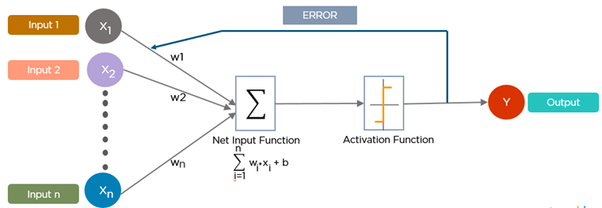
\includegraphics[width=.7\textwidth]{nn_model}
    \caption{\textit{Neural Network Model}}
    \label{fig:nn_model}
\end{figure}

This method can be applied to, for example, function approximation, classification, regression analysis, pattern recognition and decision making including more. After the learning process all that is left is a "model" or a function. This function is not a "normal" function, but a quite complex and unreadable function. But it's still a function.

\subsection{Traditional AI vs. Neural Networks}


\subsection{Types of Neural Networks}
There are mainly three major learning paradigms in neural networks: Reinforcement Learning, Supervised Learning and Unsupervised Learning.

% https://scikit-learn.org/stable/tutorial/basic/tutorial.html#machine-learning-the-problem-setting (this explains very vell these three types.):
\subsubsection{Reinforcement Learning}
\subsubsection{Supervised Learning}
\subsubsection{Unsupervised Learning}

\subsection{Single Neuron}
\subsection{Deep Learning}


NOTES:
* The weight of the edges might have a threshold, so that if the connection exceeds the threshold, the signal gets sent.
* Often the nodes are aggregated into layers

* image classification (goal: to train a model to be able to classify images that it has never seen before)
	* predict what the image is (what type of clothing) from 0 - 10
	* goal: to get low 'evidence' of all other clothing, and high 'evidence' of the one that it is (for example nr 7)
	* after training we will look at what the network predicted compared to what it actually is in the training example. The resulting number we get here is what is called 'loss'. (which is a fancy word for error). (Loss function)
	* then the network is optimising itself to reduce the loss.

* Training set and testing set (supervised learning)

* Normalisation/prepossessing data before feeding into the network
* the first layer is only prepossessing the data and is not actually doing any calculations.

Build the model:
	* configuring the layers of the model
	* compiling the model (AdamOptimizer)
	* test the model
		* Evaluate the accuracy between the training and the testing
          * Here we get a number: 'test accuracy'
          * We now only care that the 'test accuracy' is very similar to the accuracy from the training section.
              * If these numbers are very similar, we can conclude that the 'Epoch' number (how long the training will last for was set to a sensible number - in this case it was set to 5.
              * If the 'test accuracy' is lower than the 'training accuracy' then we can conclude that we overfit the network, or we trained it for too long.
              * If both numbers are low, this means that we have not trained the network for too long.
          * So the way we find the number of epochs is you run experiments (train over and over again)
          * A prediction is an array of 10 numbers. These describe the confidence of the model that the image corresponds to each of the 10 different articles of clothing.

* activation function / transfer function / system function / network function

There are NNs that work with 2D images - convolutional networks (check out later)

* Overfitting vs. Underfitting (memorization vs generalization)
    * if we train the network too short a time, the network will not be very good at classifying data and it woun't have learned enough patterns
    * if we train the network too long a time, the network will learn overly specific patterns and it will start to memorise the training-data itself.
    * We want to find the sweet spot so that the resulting model has a good understanding of the possible patterns in a generalised way.

* NNs can either be 'feed forward' or 'cyclic or recurrent'

Look into KNN and Decision Trees, and then into the 'black box' land of neural networks.

% END NOTES

\subsection{Feedfoward Network & Dense Layer & Dropout Network}
"In this type of architecture, a connection between two nodes is only permitted from nodes in layer i to nodes in layer i + 1 (hence the term feedforward; there are no backwards or inter-layer connections allowed). NOTE: The arrows are all moving in one direction." (https://www.quora.com/In-TensorFlow-what-is-a-dense-and-a-dropout-layer)

“A dense layer is a fully connected layer, as in, all neurons in the previous layer are connected to all neurons in the next layer.“

% Decision Trees & kNN
\subsection{Decision Trees & kNN}
% https://scikit-learn.org/stable/modules/tree.html#decision-trees

% Backpropagation

\begin{quote}
    \textit{"The honeymoon is officially over, and neural computing has moved beyond simple demonstrations to more significant applications."} (Sharkey, 1999)
\end{quote}

\begin{quote}
    \textit{"It has been shown that the robustness and reliability of an ANN (artificial neural network) can be often significantly improved by appropriately combining several ANN models into an ANN ensemble. The construction of such an ensemble requires two main steps. The first is to create individual ensemble members, and the second is to find the appropriate combination of outputs from those members for producing the unique ensemble output."} (Linares-Rodriguez, Ruiz-Arias, Pozo-Vazquez, & Tovar-Pescador, 2013)
\end{quote}

In this experiment [cite], the goal was to obtain more reliable results in regards to estimating global solar radiation from satellite images by combining the ANNs. The results from the five best models that were selected were compared. Now, after analyzing the data given, an ANN-ensemble of these individual ANNs were constructed and built.

This demonstrates just how combining models can outperform individuals. This can lessen the overall bias to any specific model, hence make the ensemble more fair and reliable.



% Simulations

According to Woodford & Plessis (2018), performing experiments in a virtual world or a simulation, often helps us speed up the process of learning artificial neural networks.
\begin{quote}
    \textit{"The evaluation of many controllers is typically performed in a simulation instead of real-world in order to speed up the evolutionary process."} [...] (Woodford & Plessis, 2018).
\end{quote}
* Traditional AI vs. Neural networks
* Neural Networks: RL, SL, USL, Other Algorithms

\begin{quote}
    \textit{"Neurons that fire together, wire together."}
\end{quote}


\clearpage


%----------------------------------------------------------------------------------------
%	ENSEMBLE NEURAL NETWORKS
%----------------------------------------------------------------------------------------
\section{Ensemble Neural Networks}
% https://scikit-learn.org/stable/modules/ensemble.html (Great descriptions)
Ensemble Learning is a method within the field of Machine Learning where one tries to combine several models. This can help to obtain a result or output that is less bias, more accurate, decreased variance and better predictive performance. According to Medium (10105510377845702, 2017) by having people use ensemble methods get's placed first in many prestigious machine learning competitions, such as the Netflix Competition, KDD 2009, and Kaggle.

\begin{quote}
    \textit{"The idea of ensemble learning methods is to select a collection, or ensemble, of hypotheses from the hypothesis space and combine their predictions."} (Russell, 2018)
\end{quote}

* Variance \& Bias
\begin{quote}
    \textit{"Normally, as you increase the complexity of your model, you will see a reduction in error due to lower bias in the model. However, this only happens till a particular point. As you continue to make your model more complex, you end up over-fitting your model and hence your model will start suffering from high variance. "}
\end{quote}
    
    * Bagging, Boosting
* General: Previous ensembles to simulations or other applications?
* Specific: Previous ensembles that have been applied to a snake game

\subsection{Ensemble Learning Examples}


\section{Computer Simulations}
\subsection{Speedup}


%----------------------------------------------------------------------------------------
%	CHAPTER 3: METHODOLOGY
%----------------------------------------------------------------------------------------
\chapter{Methodology}
% Explain and discuss all methods and options considered, and justify the ones been used.
% NOTES: PPO, and other algorithms. Over- Underfitting.

\section{Overview}
In order to proceed with the project, numerous applications, methods, languages, tools, libraries, algorithms and technologies were considered. The various methodologies were briefly described, discussed and justified in order to select the most appropriate ones in accordance with the task at hand.

\section{Project Management}
\subsection{Applications}
\section{Software Development Methodologies}
\section{Languages}
\section{Libraries}
\section{Snake Games}
\subsection{Game Changes}
\section{Algorithms}
Policy Network\\
Proximal Policy Optimization\\
Cross Entropy Algorithm\\
Very useful article: https://medium.com/coinmonks/landing-a-rocket-with-simple-reinforcement-learning-3a0265f8b58c



%----------------------------------------------------------------------------------------
%	CHAPTER 4: SOLUTION IMPLEMENTATION
%----------------------------------------------------------------------------------------
\chapter{Solution Implementation}

A Beginner's Guide to Deep Reinforcement Learning: https://skymind.ai/wiki/deep-reinforcement-learning
(include as section) No Free Lunch Theorem (https://www.youtube.com/watch?v=itgRZDurMlc) - must include

\section{Overview}
% Justification for Creating the Snake Game by scratch
    % game loop (continuous) vs command-line-interface (step by step). Game vs Simulation
    % references
    % many good games implemented in python, but
    % needed a game to communicate with Model
    % and receiving commands from the Model
    % save all snapshots from every game-state
    % save all games
In order to achieve the prepared deliverables, there needs to be implemented several modules in the system. Some of the modules are:

\begin{myitemize}
    \item environment
    \item brain
    \item snake
    \item communicator
\end{myitemize}

The environment in our system is the game or simulation, the brain is the artificial neural network, the snake is an Agent and the communicator is what is called an API. In order to make this system, we are dependent on an environment, meaning this needs to be implemented before any other module.

\begin{figure}[h]
    \centering
    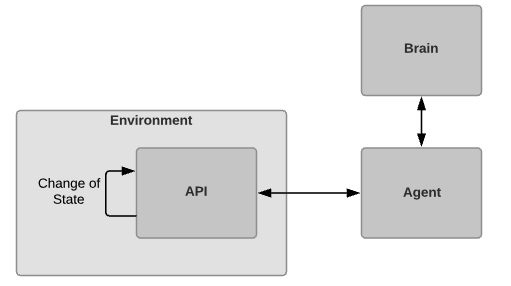
\includegraphics[width=.7\textwidth]{overview}
    \caption{\textit{The environment is the game, also holding an interface. This let's ideally any Agent-type influence or alter the environment.}}
    \label{fig:overview}
\end{figure}

There were set off time to look for multiple possible implementations of the Snake Game that could work for our plan. Multiple games were considered strongly. See references (TODO: include refs). However, after all consideration, it was decided that the game needed to be implemented from scratch. The reason for this is manifold:

\begin{myitemize}
    \item Provide flexible and appropriate data to the Network
    \item Communication between Game and Network
    \item Continuous and not step-by-step
    \item Spaghetti-Code
    \item Debugging
\end{myitemize}

To be able to provide flexible and appropriate data to the network, one have to have this in mind while designing the game from the ground up. Many of the games that was inspected had some data, but not necessarily for instance every \textit{state} of every \textit{move} of every \textit{game}, therefore not being flexible enough. Also some games provided irrelevant and data that was not required.

To be able to communication between the game and the network, one often needs an API. This could have been implemented in any Snake game, but was rather designed along with the game itself to make sure all design principles were followed.

The game needed to have a step-by-step design instead of a continuous classical game-loop. A continuous game-loop is not needed as the data being processed should go as quick as possible (no need for delay to let any human see the game) considering no human should ever play the game and also no printing will occur (at least not during the training as this sadly will increase the speed immensely). If at a later point a human should interact and possibly compete with the agent, a human-version can also be made as another branch in the future.

\section{Snake Game Design \& Implementation}

\subsection{Game Loop}
When the agent wants to do an action onto the environment it will request a direction to receive from the Brain. Once the agent holds a current direction it wants to move in ('up','down','right','left'), it will act upon the environment by sending a move command: \textit{update('right')} to the game-simulation. The game will be updated, and as long as the game is not over, it will continue until one of the following: the agent moves outside the board, the agent moves into itself, or if the agent happens to \textit{'loop'} in a certain route on the board. Hence we need a timeout most likely.

\begin{figure}[h]
    \centering
    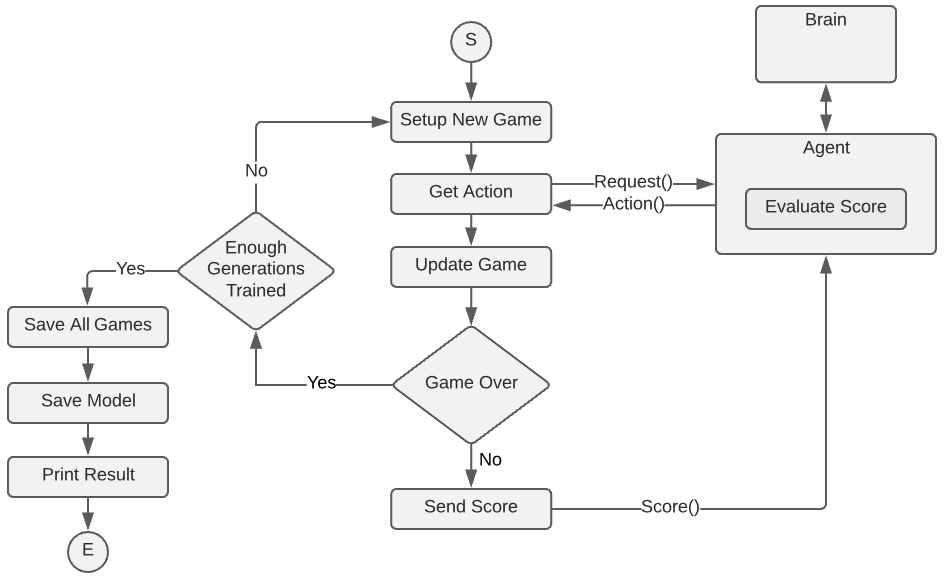
\includegraphics[width=.75\textwidth]{game_loop}
    \caption{\textit{Game Loop}}
    \label{fig:game_loop}
\end{figure}

If the current game happens to end, the system will immediately add that game to a list: \textit{all\_games} and then start a new game unless the achieved number of generations is reached. When the number of generations is reached, the system will end with saving the list of all\_games and the model/function as well as printing an overview to the console and to a log-file.

\subsection{Class Diagram}
\begin{figure}[h]
    \centering
    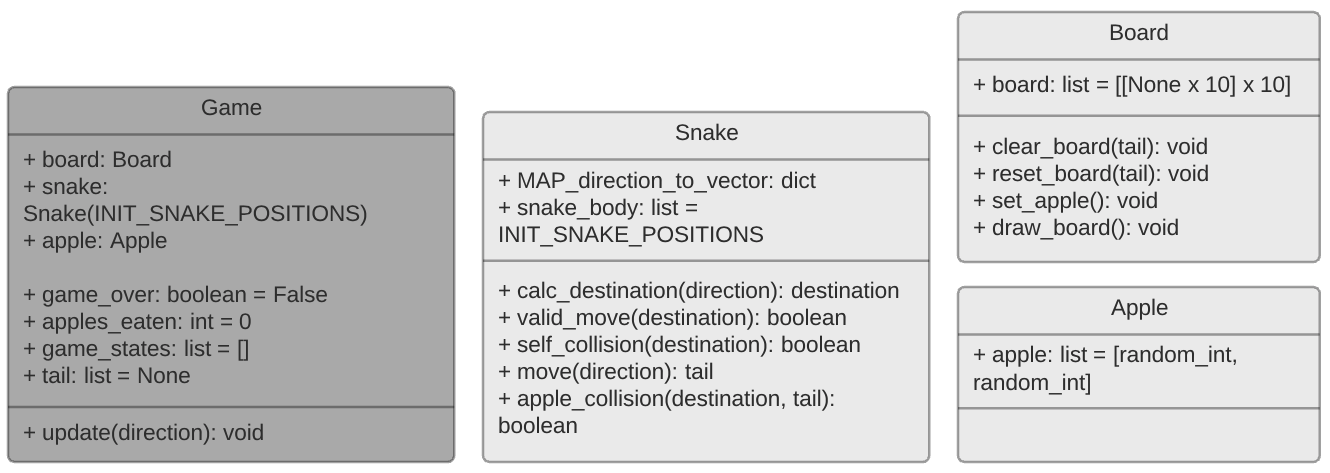
\includegraphics[width=.9\textwidth]{game_class_diagram}
    \caption{\textit{The Game is holding a Board, a Snake and an Apple}}
    \label{fig:game_class_diagram}
\end{figure}

\subsubsection{Modular Design}
Compliant with cloud computing and distributed systems, multi agent systems, multiple servers, scaleable...

\section{Model Implementation}
Now that we have the environment implemented, our next step is to implement the Agent and it's Brain. The Brain of the Agent is the system that is responsible for providing the best actions to the agent to let it act upon the environment. This is what is known as reinforcement learning.

\subsection{Reinforcement Learning}
So as discussed, both supervised and unsupervised learning is all about pattern recognition. Classifying or clustering data, predicting for instance what an object is on a given image, given some possible labels. However, in reinforcement learning, it is more about trial-and-error. And instead of using labels, we want to use rewards to train our agent. This interests us more as supervised learning needs lots of training data, possibly from a human player, to try and mimic that player, never really achieving any higher score than that player itself does. Rather, we want to optimize the game as much as possible, hence we want to look at what options we have for reinforcement learning, but first we will look at Markov Decision Process which is a central concept in reinforcement learning.

\subsubsection{Markov Decision Process}
Looking closer at the Markov Decision Process in Figure \ref{fig:markov_decision_process}, we can actually understand that both the Agent and the Environment are indeed just functions for one another. The environment takes an action as an input and outputs both a state and a reward, while the Agent takes that data (state and reward) and gives back an action again. However it is important to understand that the environment function is indeed the function that the Agent is trying to predict or mimic, hence this is the unknown function that we will try to approximate.

In any Markov Decision Process there are usually 5 important properties:

\begin{myitemize}
    \item States
    \item Model
    \item Actions
    \item Reward
    \item Policy
\end{myitemize}

\begin{figure}[h]
    \centering
    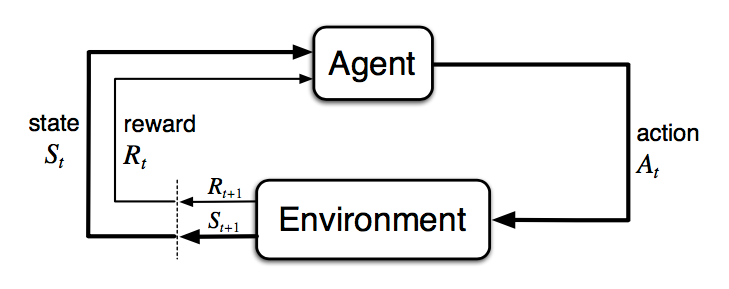
\includegraphics[width=.65\textwidth]{markov_decision_process}
    % \caption{Markov Decision Process: The environment is often referred to as a black-box. This just means that the environment function is unknown and the only thing we can see is the input and output. Source: [12] https://skymind.ai/wiki/deep-reinforcement-learning}
    \label{fig:markov_decision_process}
    \caption{\textit{Markov Decision Process}}
\end{figure}

In any interaction of a simulation that the agent takes upon the environment, will occur sequentially over time, feeding back the state of the environment to the agent. It is just a simple loop, just like the game-loop already implemented.

\begin{quote}
    \textit{"Reinforcement learning represents an agent’s attempt to approximate the environment’s function, such that we can send actions into the black-box environment that maximize the rewards it spits out."} (A Beginner's Guide to Deep Reinforcement Learning).
\end{quote}

In reinforcement learning it is important to explore the environment first to let the agent get a basic understanding of what actions gives a good reward and what actions can give back a negative reward or a penalty. Doing this will hopefully make the agent learn quickly. This is why we often set the whole matrix or tensor to be completely random numbers initially and then for each step of the game-loop the agent tweaks these values iteratively.

We have to be able to in any state of the game, get the reward or score of the current state, as well as getting the state itself of the present game. Let's break it down:

\subsubsection{Reward}
The reward will be calculated by the environment, telling the agent how good the current state is and how well it performed. In our example if the snake-agent is moving towards an apple, the agent can understand this by getting a 'treat'. If the agent touches the apple it get a high reward, and if it get'
s closer to the apple, it can for example get the score of the apple divided by the length to the apple.

\subsubsection{State}
The current state of the game will also be sent from the environment to the agent. This is what the agent will feed the Brain, hence making the it interpret the best action to take for the agent.

Providing these two datasets is the environment's responsibility which we have already implemented in the game.


...

\subsection{Tensorflow}
What is a scalar vs vector vs matrix vs tensor.
Why did I use Tensorflow?

\begin{figure}[h]
    \centering
    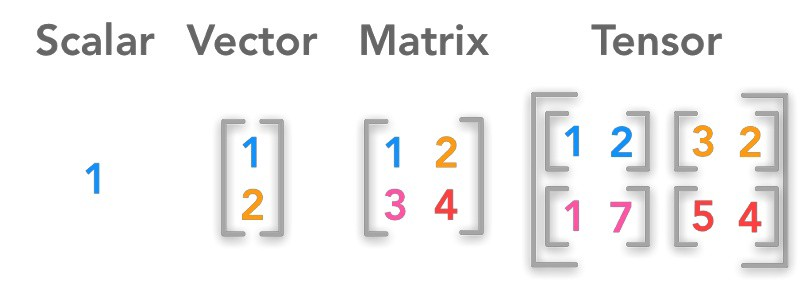
\includegraphics[width=.7\textwidth]{tensor}
    \caption{\textit{Tensor}}
    \label{fig:tensor}
\end{figure}

\subsection{Q-learning}
% [ ] White Paper: https://web.stanford.edu/class/psych209/Readings/MnihEtAlHassibis15NatureControlDeepRL.pdf
% [ ] White Paper: https://onlinelibrary.wiley.com/doi/pdf/10.1002/int.20105 \newline
% [ ] White Paper: https://ieeexplore.ieee.org/document/7849368
Q-learning was considered strongly in this project. The reason for this are manifold. First, this algorithm have gotten a lot of praise recently. It has even been shown to be able to in some cases approach general artificial intelligence as the agent developed in this study (Mnih, et al., 2015) was able to play 50 different Atari Games as well as achieve superhuman performance in all of them.

Secondly, this technique has also been shown to be able to be implemented in a neural network too. This makes it a beginner friendly method as complexity can further be added.

\begin{quote}
    "Q-learning is a simple way for agents to learn how to act optimally in controlled Markovian domains. It amounts to an incremental method for dynamic programming which imposes limited computational demands. It works by successively improving its evaluations of the quality of particular actions at particular states." (Watkins & Dayan, 1992)
\end{quote}

The Q-learning algorithm is a reinforcement learning algorithm. Its overall goal is to find an optimal policy in order to act upon the environment in a desired manner to get the most reward. The algorithm uses a matrix or a look-up table often referred to as the \textit{Q-table}. Each row in the table holds the state with each column representing the actions. Each value in the table is referred to as a \textit{Q-value}. The Q-values represent the expected \textit{reward} that the agent will receive by taking that action. These values can be initialized randomly or as zero, or Null-int32-values (signed integer) as the value can range from positive to negative.

The variables most often seen in Q-learning are:

\begin{myitemize}
    \item Q-table
    \item Q-values (expected reward from action in a given state)
    \item Epsilon: random- vs learned actions trade off
    \item Discount Rate: short- vs long term reward trade off
    \item Target Value: the final Q-table
    \item Learning Rate: how aggressively to apply new knowledge
\end{myitemize}

\begin{figure}[h]
    \centering
    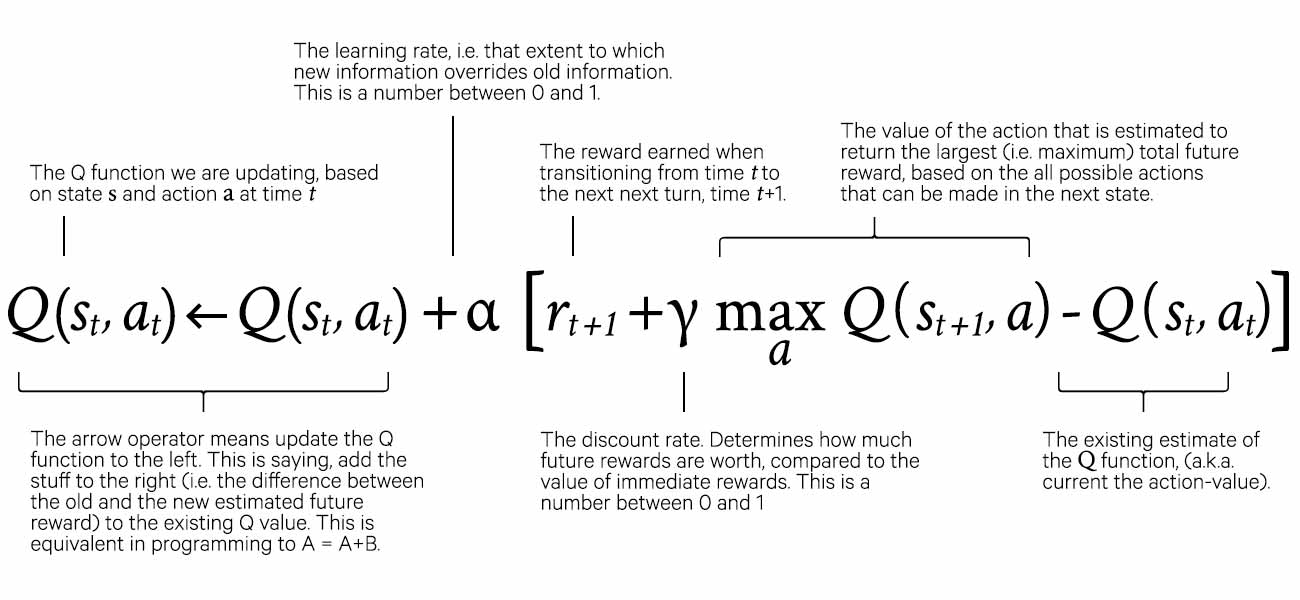
\includegraphics[width=.95\textwidth]{q_learning_algorithm}
    \caption{\textit{Q-learning Algorithm:} Source: https://randomant.net/reinforcement-learning-concepts/}
    \label{fig:q_learning_algorithm}
\end{figure}

\subsubsection{Q-table \& Q-values}
The Q-table is a simple matrix. The rows are all possible states, and the columns are the actions. The Q-values will be initialized randomly, and we will approximate them by tweaking these values depending on the reward given.

\subsubsection{Epsilon}
The \textit{epsilon} value makes it so that the agent don't value that reward as much in the very beginning. This is because in the start we want to value random decisions more, simply to \textit{explore} the environment and what actions lead to which rewards. Later, as we learn more and more the epsilon will decrease, to favor more the actual knowledge the agent has over random actions. This is what is know as the exploration vs. exploitation trade-off.

\subsubsection{Discount Rate}
The discount rate is just a scalar that is applied to each reward. Since the environment is unpredictable or non-deterministic, this value is added on each reward exponentially, as the rewards further into the future is more likely to diverge. So the more into the future the reward is, the less we take it into account.

\subsubsection{Target Value}
The target value is the value we always want to achieve. This value is simply the best possible sequence of rewards we can get being in a given state.

\begin{quote}
    \textit{"The maximum future reward for this state and action, is the immediate reward plus the maximum future reward for the next state. This is also called the Bellman Equation"} (youtube video: https://www.youtube.com/watch?v=79pmNdyxEGo)
\end{quote}

\subsubsection{Learning Rate}
This scalar is simply how fast we want the agent to apply the new knowledge it is learning. This is often referred to as the $\alpha$ alpha-learning rate, and in practice often is a constant of about 0.1 or 0.2. This means it will value mostly what it already knows, but reapply or override this a little bit.

\subsection{Convolutional Neural Network (CNN)}
Future work? Make the algorithm work by seeing the pixels in any given game. This is so that we can approach a general method to play any game.

\subsection{OpenAI Gym: Frozen Lake}
To familiarize ourselves, the OpenAI-gym library was used. OpenAI has an extensive library of a range of both discrete and continous games availiable for developers to use. The environments are made purposely to apply ML techniques with a shared interface. One of the environments they have are very similar to the problem domain we are having.

FrozenLake is a classical game where the problem is to simply move a node (in our case the snake head) on a grid towards a randomly selected location (where the apple is).


%----------------------------------------------------------------------------------------
%	CHAPTER 5: EVALUATION & TESTING
%----------------------------------------------------------------------------------------
\chapter{Testing \& Evaluation}

%----------------------------------------------------------------------------------------
%	CHAPTER 6: CONCLUSION & FUTURE WORK
%----------------------------------------------------------------------------------------
\chapter{Conclusion \& Future Work}

...


% Learning Outcomes
% 1. Manage a substantial individual project, including planning, documentation and control.
% 2. Construct a focused problem statement and conduct a suitable investigation, including literature or technology review, into the context of that problem
% 3. Demonstrate professional competence by applying appropriate theory and practice to the analysis, design, implementation and evaluation of a non-trivial set of deliverables.
% 4. Show a capacity for self-appraisal by analysing the strengths and weaknesses of the project process and outcomes with reference to the initial objectives and to the work of others.
% 5. Provide evidence of the foregoing in the form of a report.
% 6. Defend the work orally at a Viva Voce examination and by means of a poster presentation.




% Questions:
% Q1: Can I write about things I know without 'always' looking it up from different sources if I know the topic? Or should I always refer to a source? (I refer most of the time though)
% Q2: Can I include sections from my IPO in my thesis, or is this strictly forbidden?
% Q3: In the learning outcomes it sais: "... including literature or technology review ...", so I should choose one or the other?
% How to present the references both in-text-citation and in ref-section?
% Should I write all text in past tens?
% Can we go over all sections, and see if I have forgotten any topic to be included in the thesis?

\chapter*{References}
\noindent [1] Sharkey, A. J. (1999). Combining artificial neural nets ensemble and modular multi-net systems. London: Springer.

\noindent [2] Linares-Rodriguez, A., Ruiz-Arias, J. A., Pozo-Vazquez, D., & Tovar-Pescador, J. (2013). An artificial neural network ensemble model for estimating global solar radiation from Meteosat satellite images. Energy, 61, 636-645. Retrieved January 8, 2019, from https://www.sciencedirect.com/science/article/pii/S0360544213007597#cebib0010.

\noindent [3] Woodford, G. W., & Plessis, M. C. (2018). Robotic snake simulation using ensembles of artificial neural networks in evolutionary robotics. Proceedings of the Genetic and Evolutionary Computation Conference on - GECCO 18, 61, 636-645. doi:10.1145/3205455.3205507

\noindent [4] Russell, S. N. (2018). Artificial Intelligence: A modern approach. Place of publication not identified: Pearson.

\noindent [5] 10105510377845702. (2017, August 22). Ensemble Learning to Improve Machine Learning Results. Retrieved January 8, 2019, from https://blog.statsbot.co/ensemble-learning-d1dcd548e936

\noindent [6] O'Malley, J. (2018, January 10). The 10 most important breakthroughs in Artificial Intelligence. Retrieved from https://www.techradar.com/news/the-10-most-important-breakthroughs-in-artificial-intelligence

\noindent [7] Copeland, B. (2018, August 17). Artificial intelligence. Retrieved from https://www.britannica.com/technology/artificial-intelligence

\noindent [8] Watson, I. (2012, April 26). How Alan Turing Invented the Computer Age. Retrieved from https://blogs.scientificamerican.com/guest-blog/how-alan-turing-invented-the-computer-age/

\noindent [9] Benefits & Risks of Artificial Intelligence. (n.d.). Retrieved from https://futureoflife.org/background/benefits-risks-of-artificial-intelligence/?cn-reloaded=1

\noindent [10] Harari, Y. N. (2016). Homo deus. Place of publication not identified: Harvill Secker.

\noindent [11] Bossmann, J. (n.d.). Top 9 ethical issues in artificial intelligence. Retrieved from https://www.weforum.org/agenda/2016/10/top-10-ethical-issues-in-artificial-intelligence/

\noindent [12] A Beginner's Guide to Deep Reinforcement Learning. (n.d.). Retrieved from https://skymind.ai/wiki/deep-reinforcement-learning

\noindent [13] Watkins, C. J., & Dayan, P. (1992). Technical Note. Reinforcement Learning, 55-68. doi:10.1007/978-1-4615-3618-5_4

\noindent [14] Mnih, V., Kavukcuoglu, K., Silver, D., Rusu, A. A., Veness, J., Bellemare, M. G., . . . Hassabis, D. (2015). Human-level control through deep reinforcement learning. Nature,518(7540), 529-533. doi:10.1038/nature14236

\chapter*{Appendix}

\end{document}
